\subsubsection{Macro-caso d'uso - Gestione Materiali}
\paragraph{Diagramma UML}

\begin{figure}[H]
    \centering
    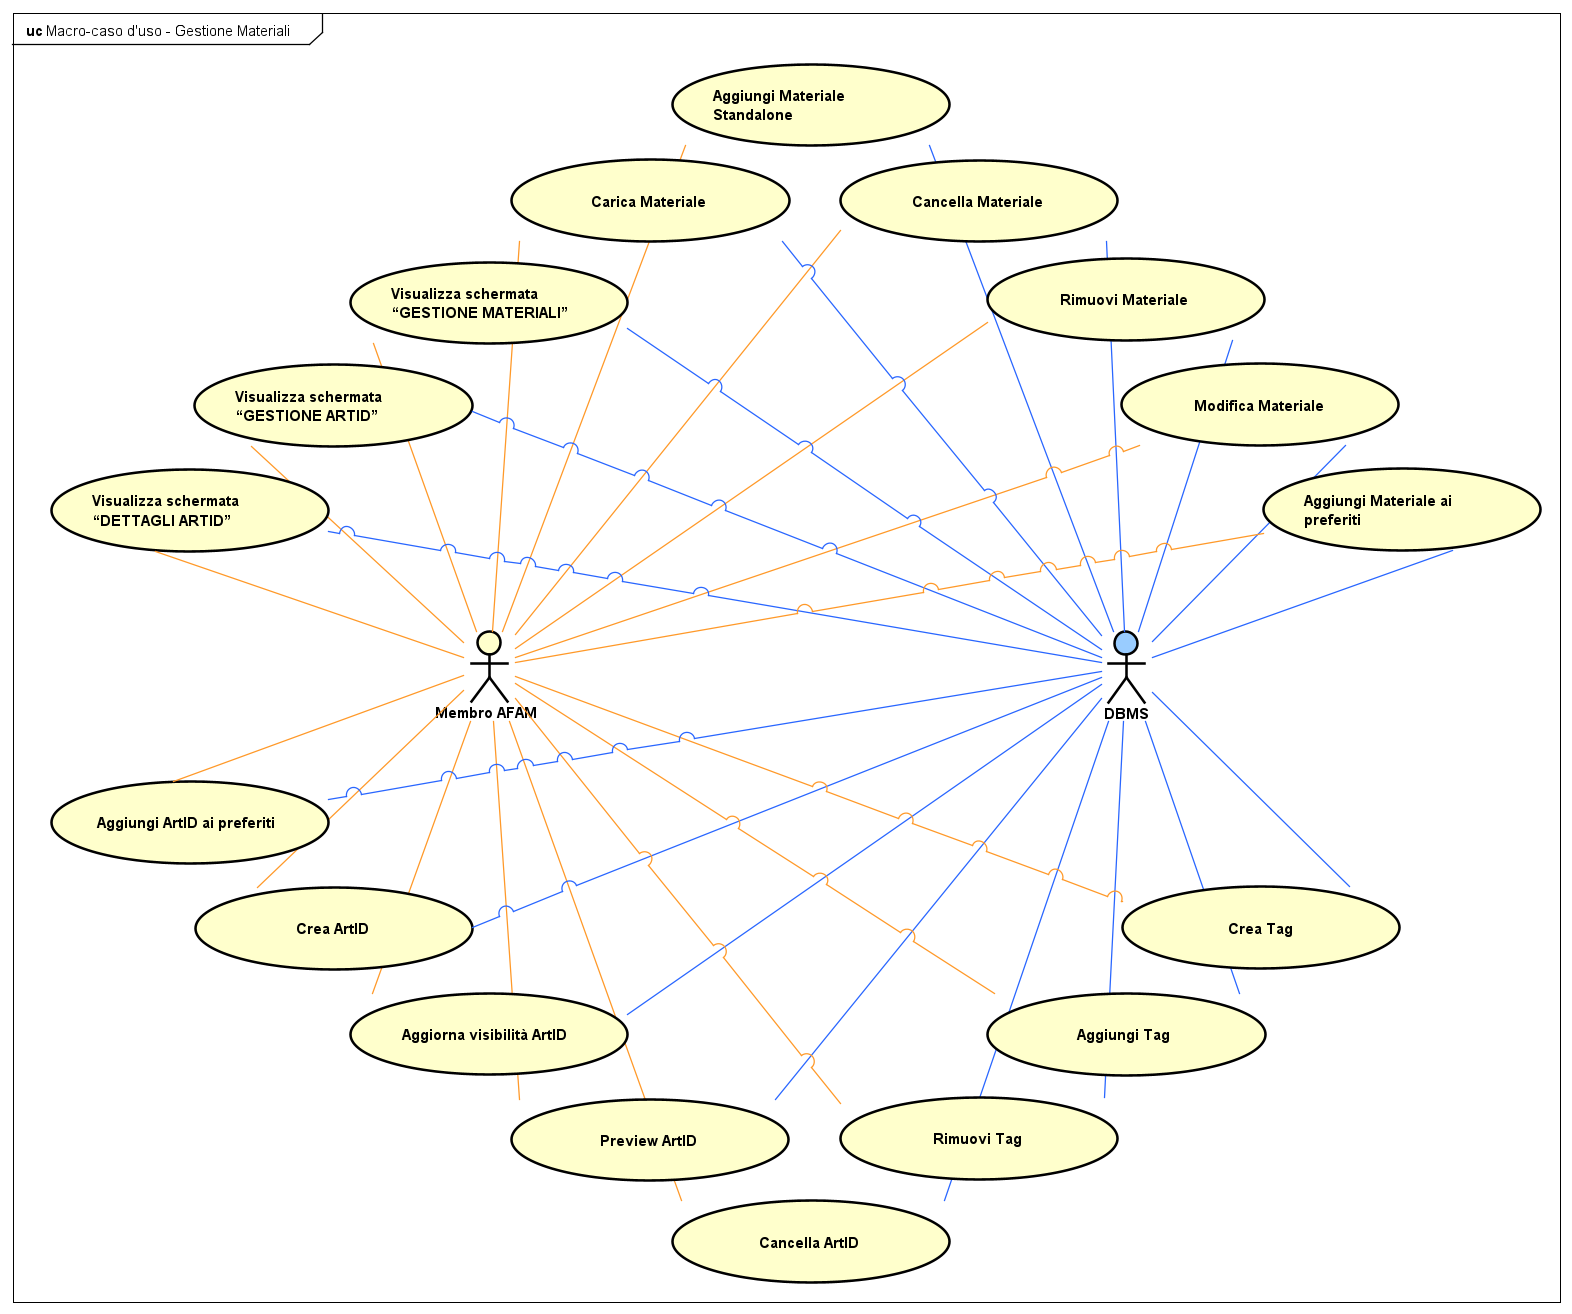
\includegraphics[width=0.95\textwidth, height=0.95\textheight, keepaspectratio]{Immagini/Use-case diagrams/Macro-caso d'uso - Gestione Materiali.png}
\end{figure}

\clearpage

\paragraph{Visualizza schermata ``GESTIONE ARTID''}
\par{ \noindent  Il seguente caso d'uso permette di visualizzare tutti gli ArtIID del Membro AFAM.\\
\`E prevista la creazione e cancellazione di ArtID da poter condividere.}

\begin{tabularx}{\textwidth}{|C|X|}
\hline
\rigaTabella{Caso d'uso}{Visualizza schermata ``GESTIONE ARTID''}
\rigaTabella{ID}{VIS\_SCH\_GES\_ARTID}
\rigaTabella{Attori}{Membro AFAM, DBMS}
\rigaTabella{Precondizione}{Il sistema ha mostrato a video la ``HOME''}
\rigaTabella{Flusso degli eventi}{\begin{enumerate}
    \item Il Membro clicca sul bottone ``ARTID''
    \item Il sistema interroga il DBMS per ottenere tutti gli ArtID del Membro
    \item Il sistema mostra a video la schermata ``GESTIONE ARTID'' che contiene tutti gli ArtID del Membro
\end{enumerate}
}
\rigaTabella{Postcondizione}{Il sistema ha mostrato a video la schermata ``GESTIONE ARTID'' che contiene tutti gli ArtID del Membro}
\rigaTabella{Note}{Opzionalmente il Membro può filtrare la lista degli ArtID a schermo cliccando sui bottoni laterali.
I filtri sono ``I miei'', ``Condivisi con me'', ``Recenti'', ``Preferiti''}
\hline
\end{tabularx}

\paragraph{Visualizza schermata ``GESTIONE MATERIALI''}
\par{\noindent Il seguente caso d'uso permette di visualizzare tutti i materiali del Membro AFAM.\\
\`E previsto l'inserimento e la cancellazione di materiali.}

\begin{tabularx}{\textwidth}{|C|X|}
\hline
\rigaTabella{Caso d'uso}{Visualizza schermata ``GESTIONE MATERIALI''}
\rigaTabella{ID}{VIS\_SCH\_GES\_MAT}
\rigaTabella{Attori}{Membro AFAM, DBMS}
\rigaTabella{Precondizione}{Il sistema ha mostrato a video la ``HOME''}
\rigaTabella{Flusso degli eventi}{\begin{enumerate}
    \item Il Membro clicca sul bottone ``MATERIALI''
    \item Il sistema interroga il DBMS per ottenere tutti i materiali del Membro
    \item Il sistema mostra a video la schermata ``GESTIONE MATERIALI'' che contiene tutti i materiali del Membro
\end{enumerate}
}
\rigaTabella{Postcondizione}{Il sistema ha mostrato a video la schermata ``GESTIONE MATERIALI'' che contiene tutti i materiali del Membro}
\rigaTabella{Note}{Opzionalmente il Membro può filtrare la lista dei Materiali a schermo cliccando sui bottoni laterali.
I filtri sono per tipo di materiale [es. audio, video], recenti e preferiti.}
\hline
\end{tabularx}

\clearpage

\paragraph{Visualizza schermata ``DETTAGLI ARTID''}
\par{\noindent Il seguente caso d'uso permette di visualizzare tutti i dettagli dell'ArtID selezionato. \\ 
\`E prevista la possibilità di aggiungere Materiali e Tag, di aggiungere o rimuovere dai preferiti l'ArtID e di condividerlo.}

\begin{tabularx}{\textwidth}{|C|X|}
\hline
\rigaTabella{Caso d'uso}{Visualizza schermata ``Gestione ArtID''}
\rigaTabella{ID}{VIS\_SCH\_GES\_ARTID}
\rigaTabella{Attori}{Membro AFAM, DBMS}
\rigaTabella{Precondizione}{Il sistema ha mostrato a video la schermata ``GESTIONE ARTID''}
\rigaTabella{Flusso degli eventi}{
    \begin{enumerate}
        \item Il Membro clicca l'ArtID che vuole visionare
        \item Il sistema interroga il DBMS per ottenere tutte le informazioni dell'ArtID
        \item Il sistema mostra la schermata ``DETTAGLI ARTID''
    \end{enumerate}
}
\rigaTabella{Postcondizione}{Il sistema ha mostrato a video la schermata ``DETTAGLI ARTID'' che contiene tutte le informazioni dell'ArtID}
\end{tabularx}

\clearpage

\paragraph{Carica Materiale}
\par{\noindent Questo caso d'uso permette al Membro AFAM di caricare i propri materiali multimediali.}

\begin{tabularx}{\textwidth}{|C|X|}
\hline
\rigaTabella{Caso d'uso}{Carica Materiale}
\rigaTabella{ID}{CRE\_MAT}
\rigaTabella{Attori}{Membro AFAM, DBMS}
\rigaTabella{Precondizione}{Il sistema ha mostrato a video la schermata ``GESTIONE MATERIALI''}
\rigaTabella{Flusso degli eventi}{\begin{enumerate}
    \item Il Membro clicca sul pulsante ``NUOVO''
    \item Il sistema mostra la modale ``NUOVO MATERIALE''
    \item Il Membro inserisce il titolo e opzionalmente una descrizione del Materiale che sta per caricare
    \item Il Membro clicca sul riquadro per caricare il Materiale
    \item Il sistema mostra l'esplora file del dispositivo su cui si trova il Membro
    \item Il Membro seleziona il Materiale da caricare
    \item Il Membro clicca il tasto ``SALVA'' \label{clicca salva}
    \item Il sistema interroga il DBMS per inserire il Materiale
    \item Il sistema interroga il DBMS per ottenere la lista dei Materiali aggiornata
    \item Il sistema mostra a video la schermata ``GESTIONE MATERIALI'' con la lista dei Materiali aggiornata
\end{enumerate}
}
\rigaTabella{Sequenze alternative}{
\begin{enumerate}[start=4]
    \item Il Membro trascina il file direttamente dentro la schermata ``NUOVO MATERIALE''
    \item Il flusso riprende dal punto \ref{clicca salva} del flusso principale
\end{enumerate}
}
\rigaTabella{Postcondizione}{Il sistema ha mostrato a video la schermata ``GESTIONE MATERIALI'' aggiornata}
\rigaTabella{Requisiti Speciali}{I formati dei file che il Membro pu\`o inserire sono rigidamente limitati a: [PDF, mp4, png, jpg].}
\rigaTabella{Note}{Il pulsante ``SALVA'' \`e disabilitato se il campo titolo \`e vuoto. \newline Opzionalmente il Membro pu\`o selezionare gli ArtID in cui inserire il Materiale attraverso un apposito menu a tendina. \newline Opzionalmente il Membro pu\`o aggiungere ai preferiti il Materiale attraverso un apposito bottone.}
\hline
\end{tabularx}

\clearpage

\paragraph{Cancella Materiale}
\par{\noindent Questo caso d'uso permette al Membro AFAM di cancellare definitivamente uno o pi\`u materiali caricati sulla piattaforma.}

\begin{tabularx}{\textwidth}{|C|X|}
\hline
\rigaTabella{Caso d'uso}{Cancella Materiale}
\rigaTabella{ID}{DEL\_MAT}
\rigaTabella{Attori}{Membro AFAM, DBMS}
\rigaTabella{Precondizione}{Il sistema ha mostrato a video la schermata ``GESTIONE MATERIALI''}
\rigaTabella{Flusso degli eventi}{\begin{enumerate}
    \item Il Membro seleziona uno o pi\`u Materiali che vuole cancellare
    \item Il Membro clicca il pulsante ``CANCELLA''
    \item Il sistema mostra a video un messaggio con scritto ``Sei sicuro di voler cancellare i materiali selezionati? [listaMaterialiSelezionati]''
    \item Il Membro clicca il pulsante ``CONFERMA''
    \item Il sistema interroga il DBMS per cancellare i Materiali selezionati e aggiornare gli ArtID che lo contenevano
    \item Il sistema interroga il DBMS per ottenere la lista dei Materiali aggiornata
    \item Il sistema mostra a video la schermata ``GESTIONE MATERIALI'' aggiornata
\end{enumerate}
}
\rigaTabella{Postcondizione}{Il sistema ha mostrato a video la schermata ``GESTIONE MATERIALI'' aggiornati}
\hline
\end{tabularx}

\clearpage

\paragraph{Modifica Materiale}
\par{\noindent Questo caso d'uso permette al Membro AFAM di modificare i dettagli, quali titolo e descrizione, di un Materiale precedentemente caricato.}

\begin{tabularx}{\textwidth}{|C|X|}
\hline
\rigaTabella{Caso d'uso}{Modifica Materiale}
\rigaTabella{ID}{UPD\_MAT}
\rigaTabella{Attori}{Membro AFAM, DBMS}
\rigaTabella{Precondizione}{Il sistema ha mostrato a video la schermata ``GESTIONE MATERIALI''}
\rigaTabella{Flusso degli eventi}{\begin{enumerate}
    \item Il Membro seleziona il Materiale di cui vuole modificare i dettagli
    \item Il Membro clicca sul pulsante ``MODIFICA''
    \item Il sistema mostra la modale ``MODIFICA MATERIALE''
    \item Il Membro inserisce il nuovo titolo e la nuova descrizione del Materiale che sta modificando
    \item Il Membro clicca il tasto ``SALVA''
    \item Il sistema interroga il DBMS per aggiornare i dettagli del Materiale
    \item Il sistema interroga il DBMS per ottenere la lista dei Materiali aggiornata
    \item Il sistema mostra a video la schermata ``GESTIONE MATERIALI'' con la lista dei Materiali aggiornata
\end{enumerate}
}
\rigaTabella{Postcondizione}{Il sistema ha mostrato a video la schermata ``GESTIONE MATERIALI'' aggiornata}
\rigaTabella{Note}{Il pulsante ``SALVA'' \`e disabilitato se il campo titolo e descrizione non sono stati modificati o se il campo titolo \`e vuoto. \newline Opzionalmente il Membro pu\`o aggiungere ai preferiti il Materiale attraverso un apposito bottone presente nella modale ``MODIFICA MATERIALE''.}
\hline
\end{tabularx}

\clearpage

\paragraph{Aggiungi Materiale ai preferiti}
\par{\noindent Questo caso d'uso permette al Membro AFAM di contrassegnare un Materiale come preferito per facilitarne l'individuazione all'interno della piattaforma, offrendo anche la possibilit\`a di rimuovere tale stato.}

\begin{tabularx}{\textwidth}{|C|X|}
\hline
\rigaTabella{Caso d'uso}{Aggiungi Materiale ai preferiti}
\rigaTabella{ID}{PREF\_MAT}
\rigaTabella{Attori}{Membro AFAM, DBMS}
\rigaTabella{Precondizione}{Il sistema ha mostrato a video la schermata ``GESTIONE MATERIALI''}
\rigaTabella{Flusso degli eventi}{\begin{enumerate}
    \item Il Membro clicca sul pulsante ``PREFERITI'' del Materiale che vuole aggiungere ai preferiti
    \item Il sistema interroga il DBMS per aggiungere il Materiale ai preferiti
    \item Il sistema interroga il DBMS per ottenere la lista dei Materiali aggiornata
    \item Il sistema mostra a video la schermata ``GESTIONE MATERIALI'' con la lista dei Materiali aggiornata
\end{enumerate}
}
\rigaTabella{Postcondizione}{Il sistema ha mostrato a video la schermata ``GESTIONE MATERIALI'' aggiornata}
\rigaTabella{Note}{Se il Materiale \`e gi\`a tra i preferiti, cliccando sul pulsante ``PREFERITI'', al Materiale verr\`a rimossa la propriet\`a.}
\hline
\end{tabularx}

\clearpage

\paragraph{Crea ArtID}
\par{\noindent Questo caso d'uso permette al Membro AFAM di creare un ArtID}

\begin{tabularx}{\textwidth}{|C|X|}
\hline
\rigaTabella{Caso d'uso}{Crea ArtID}
\rigaTabella{ID}{CRE\_ARTID}
\rigaTabella{Attori}{Membro AFAM, DBMS}
\rigaTabella{Precondizione}{Il sistema ha mostrato a video la schermata ``GESTIONE ARTID''}
\rigaTabella{Flusso degli eventi}{\begin{enumerate}
    \item Il Membro clicca sul pulsante ``NUOVO ARTID''
    \item Il sistema mostra la modale ``CREA ARTID''
    \item Il Membro inserisce il titolo dell'ArtID 
    \item Il sistema controlla il campo titolo
    \item Il Membro clicca il pulsante ``CREA''
    \item Il sistema interroga il DBMS per salvare l'ArtID creato
    \item Il sistema mostra la schermata ``DETTAGLI ARTID''
    \item Il Membro inserisce la descrizione
    \item Il Membro clicca sul pulsante ``AGGIUNGI MATERIALE''
    \item Il sistema interroga il DBMS per ottenere tutti i materiali del Membro
    \item Il sistema mostra la schermata ``AGGIUNGI MATERIALE''
    \item Il Membro seleziona uno o pi\`u materiali dalla lista dei materiali, opzionalmente, filtrando la lista compilando la barra di ricerca
    \item Il Membro clicca sul pulsante ``AGGIUNGI''
    \item Il sistema interroga il DBMS per salvare i Materiali selezionati all'ArtID
    \item Il sistema mostra la schermata ``DETTAGLI ARTID'' con i Materiali aggiunti
    \item Il Membro seleziona la visibilit\`a dell'ArtID
    \item Il sistema interroga il DBMS per aggiornare la visibilit\`a dell'ArtID
    \item Il Membro clicca sul pulsante ``SALVA''
    \item Il sistema interroga il DBMS per salvare la descrizione dell'ArtID creato
    \item Il sistema interroga il DBMS per ricevere la lista aggiornata degli ArtID
    \item Il sistema mostra a video la schermata ``GESTIONE ARTID'' con la lista degli ArtID aggiornata
\end{enumerate}
}
\rigaTabella{Postcondizione}{Il sistema ha mostrato a video la schermata ``GESTIONE ARTID'' aggiornata}
\rigaTabella{Requisiti Speciali}{I valori di visibilit\`a selezionabili dal Membro sono rigidamente definiti in: [Pubblico, Privato, Unlisted].}
\rigaTabella{Note}{Il pulsante ``CREA'' \`e disabilitato se il campo titolo \`e vuoto.}
\hline
\end{tabularx}

\clearpage

\paragraph{Aggiungi Materiale}
\par{\noindent Questo caso d'uso permette al Membro AFAM di aggiungere dei materiali presenti sulla piattaforma, ad un ArtID dopo averlo gi\`a creato.}

\begin{tabularx}{\textwidth}{|C|X|}
\hline
\rigaTabella{Caso d'uso}{Aggiungi Materiale}
\rigaTabella{ID}{AGG\_MAT}
\rigaTabella{Attori}{Membro AFAM, DBMS}
\rigaTabella{Precondizione}{Il sistema ha mostrato a video la schermata ``DETTAGLI ARTID''}
\rigaTabella{Flusso degli eventi}{\begin{enumerate}
    \item Il Membro clicca il pulsante ``AGGIUNGI MATERIALE''
    \item Il sistema interroga il DBMS per ottenere tutti i Materiali del Membro
    \item Il sistema mostra la schermata ``AGGIUNGI MATERIALE''
    \item Il Membro seleziona uno o pi\`u Materiali dalla lista dei Materiali, opzionalmente, filtrando la lista compilando la barra di ricerca
    \item Il Membro clicca sul pulsante ``AGGIUNGI''
    \item Il sistema interroga il DBMS per aggiungere i Materiali selezionati all'ArtID
    \item Il sistema mostra la schermata ``DETTAGLI ARTID'' con i Materiali aggiunti
\end{enumerate}
}
\rigaTabella{Postcondizione}{Il sistema ha mostrato la schermata ``DETTAGLI ARTID''}
\hline
\end{tabularx}

\clearpage

\paragraph{Rimuovi Materiale}
\par{\noindent Questo caso d'uso permette al membro AFAM di rimuovere dei Materiali da un ArtID.}

\begin{tabularx}{\textwidth}{|C|X|}
\hline
\rigaTabella{Caso d'uso}{Rimuovi Materiale}
\rigaTabella{ID}{REM\_MAT}
\rigaTabella{Attori}{Membro AFAM, DBMS}
\rigaTabella{Precondizione}{Il sistema ha mostrato a video la schermata ``DETTAGLI ARTID''}
\rigaTabella{Flusso degli eventi}{\begin{enumerate}
    \item Il Membro clicca sulla ``X'' accanto al Materiale che vuole rimuovere
    \item Il sistema interroga il DBMS per rimuovere il Materiale dall'ArtID
    \item Il sistema mostra a video la schermata ``DETTAGLI ARTID'' aggiornata
\end{enumerate}
}
\rigaTabella{Postcondizione}{Il sistema ha mostrato a video la schermata ``DETTAGLI ARTID'' aggiornata}
\rigaTabella{Sequenze alternative}{
\begin{enumerate}
    \item Il Membro opzionalmente clicca sulla ``X'' di un altro Materiale che vuole eliminare, il flusso riprende dal punto.
\end{enumerate}
}
\hline
\end{tabularx}

\clearpage

\paragraph{Modifica dettagli ArtID}
\par{\noindent Questo caso d'uso permette al Membro AFAM di modificare le informazioni identificative di uno specifico ArtID, inclusi il titolo, la descrizione testuale e l'immagine di copertina associata.}

\begin{tabularx}{\textwidth}{|C|X|}
\hline
\rigaTabella{Caso d'uso}{Modifica dettagli ArtID}
\rigaTabella{ID}{UPD\_ARTID}
\rigaTabella{Attori}{Membro AFAM, DBMS}
\rigaTabella{Precondizione}{Il sistema ha mostrato a video la schermata ``DETTAGLI ARTID''}
\rigaTabella{Flusso degli eventi}{\begin{enumerate}
    \item Il Membro inserisce il nuovo titolo dell'ArtID
    \item Il Membro inserisce la nuova descrizione dell'ArtID
    \item Il Membro clicca sull'immagine dell'ArtID
    \item Il sistema mostra l'esplora file del dispositivo su cui si trova il Membro
    \item Il Membro seleziona l'immagine da caricare
    \item Il Membro clicca il pulsante ``SALVA''
    \item Il sistema interroga il DBMS per aggiornare i dettagli dell'ArtID
    \item Il sistema mostra la schermata ``DETTAGLI ARTID'' aggiornata
    \item Il sistema mostra un messaggio di avvenuto aggiornamento
\end{enumerate}
}
\rigaTabella{Postcondizione}{Il sistema ha mostrato a video la schermata ``DETTAGLI ARTID'' aggiornata}
\rigaTabella{Note}{Il pulsante ``SALVA'' rimane disabilitato finch\'e almeno uno tra Titolo, descrizione o immagine non viene modificato, oppure se il campo Titolo \`e vuoto.}
\hline
\end{tabularx}

\clearpage

\paragraph{Cancella ArtID}
\par{\noindent Questo caso d'uso permette al Membro AFAM di cancellare un ArtID.}

\begin{tabularx}{\textwidth}{|C|X|}
\hline
\rigaTabella{Caso d'uso}{Cancella ArtID}
\rigaTabella{ID}{DEL\_ARTID}
\rigaTabella{Attori}{Membro AFAM, DBMS}
\rigaTabella{Precondizione}{Il sistema ha mostrato a video la schermata ``DETTAGLI ARTID''}
\rigaTabella{Flusso degli eventi}{\begin{enumerate}
    \item Il Membro clicca sul pulsante ``CANCELLA''
    \item Il sistema mostra a video un messaggio con scritto ``Sei sicuro di voler cancellare [nome ArtID]?''
    \item Il Membro clicca il pulsante ``CONFERMA''
    \item Il sistema interroga il DBMS per cancellare l'ArtID e tutti i riferimenti ai Materiali in esso contenuti e tutte le condivisioni interne ad esso riferite
    \item Il sistema interroga il DBMS per ottenere la lista degli ArtID aggiornata
    \item Il sistema mostra a video la schermata ``GESTIONE ARTID'' aggiornata
\end{enumerate}
}
\rigaTabella{Postcondizione}{Il sistema ha mostrato a video la schermata ``GESTIONE ARTID'' aggiornata}
\rigaTabella{Note}{Dopo la cancellazione di un ArtID, tutti gli eventuali link creati per condividerlo, se cliccati, mostreranno una schermata contenente un messaggio: ``L'ArtID che cerchi \`e stato cancellato''.}
\hline
\end{tabularx}

\clearpage

\paragraph{Aggiungi ArtID ai preferiti}
\par{\noindent Questo caso d'uso permette al Membro AFAM di contrassegnare un proprio ArtID come preferito per facilitarne la rintracciabilit\`a all'interno della piattaforma, offrendo anche la possibilit\`a di rimuovere tale stato.}

\begin{tabularx}{\textwidth}{|C|X|}
\hline
\rigaTabella{Caso d'uso}{Aggiungi ArtID ai preferiti}
\rigaTabella{ID}{PREF\_ARTID}
\rigaTabella{Attori}{Membro AFAM, DBMS}
\rigaTabella{Precondizione}{Il sistema ha mostrato a video la schermata ``GESTIONE ARTID'' con un qualsiasi filtro, eccetto ``CONDIVISI CON ME''}
\rigaTabella{Flusso degli eventi}{\begin{enumerate}
    \item Il Membro clicca sul pulsante ``PREFERITI'' dell'ArtID che vuole aggiungere ai preferiti
    \item Il sistema interroga il DBMS per aggiungere l'ArtID ai preferiti
    \item Il sistema interroga il DBMS per ottenere la lista degli ArtID aggiornata
    \item Il sistema mostra a video la schermata ``GESTIONE ARTID'' con la lista degli ArtID aggiornata
\end{enumerate}
}
\rigaTabella{Postcondizione}{Il sistema ha mostrato a video la schermata ``GESTIONE ARTID'' aggiornata}
\rigaTabella{Note}{Se l'ArtID \`e gi\`a tra i preferiti, cliccando sul pulsante ``PREFERITI'', all'ArtID verr\`a rimossa la propriet\`a.}
\hline
\end{tabularx}

\clearpage

\paragraph{Aggiorna visibilit\`a ArtID}
\par{\noindent Questo caso d'uso permette al Membro AFAM di modificare lo stato di visibilit\`a di un ArtID, regolando l'accessibilit\`a dei relativi link di condivisione.}

\begin{tabularx}{\textwidth}{|C|X|}
\hline
\rigaTabella{Caso d'uso}{Aggiorna visibilit\`a ArtID}
\rigaTabella{ID}{UPD\_VIS\_ARTID}
\rigaTabella{Attori}{Membro AFAM, DBMS}
\rigaTabella{Precondizione}{Il sistema ha mostrato a video la schermata ``DETTAGLI ARTID''}
\rigaTabella{Flusso degli eventi}{\begin{enumerate}
    \item Il Membro seleziona una delle opzioni di visibilit\`a dall'apposito menu a tendina
    \item Il sistema controlla l'opzione selezionata
    \item \textbf{SE} l'opzione selezionata \`e PRIVATA E precedentemente era UNLISTED ED esistono link per l'ArtID:
    \begin{enumerate}
        \item Il sistema mostra a video il messaggio: ``Questo ArtID \`e stato gi\`a condiviso, se lo rendi privato chi ha il link non potr\`a pi\`u visualizzarlo. Procedere comunque?''
        \item Il Membro clicca il tasto ``CONFERMA''
    \end{enumerate}
    \item Il sistema interroga il DBMS per aggiornare la visibilit\`a dell'ArtID 
\end{enumerate}
}
\rigaTabella{Postcondizione}{Il sistema ha mostrato a video la schermata ``DETTAGLI ARTID''}
\rigaTabella{Requisiti Speciali}{I valori di visibilit\`a da cui poter scegliere sono: [Pubblico, Privato, Unlisted]}
\rigaTabella{Note}{
    \begin{itemize}
        \item Se la visibilit\`a passa da PUBBLICA a PRIVATA, tutti gli eventuali link creati per condividerlo, se cliccati, mostreranno una pagina contenente un messaggio: ``L'ArtID che cerchi \`e privato''
        \item Se la visibilit\`a passa da UNLISTED a PRIVATA, tutti gli eventuali link creati per condividerlo, se cliccati, mostreranno una pagina contenente un messaggio: ``L'ArtID che cerchi \`e privato''
    \end{itemize}
    }
\hline
\end{tabularx}

\clearpage

\paragraph{Crea Tag}
\par{\noindent Questo caso d'uso permette di creare dei tag da aggiungere agli ArtID.}

\begin{tabularx}{\textwidth}{|C|X|}
\hline
\rigaTabella{Caso d'uso}{Crea Tag}
\rigaTabella{ID}{CRE\_TAG}
\rigaTabella{Attori}{Membro AFAM, DBMS}
\rigaTabella{Precondizione}{Il sistema ha mostrato a video la schermata ``GESTIONE ARTID''}
\rigaTabella{Flusso degli eventi}{\begin{enumerate}
    \item Il Membro clicca il pulsante ``NUOVO TAG''
    \item Il sistema interroga il DBMS per ottenere tutti i Tag del Membro
    \item Il sistema mostra la modale ``NUOVO TAG''
    \item Il Membro inserisce il nome del Tag
    \item Il sistema controlla il nome del Tag
    \item \textbf{FINCH\`E} la lunghezza del Tag \`e minore di 3 oppure il nome del Tag contiene parole vietate oppure il tag gi\`a esiste:
    \begin{enumerate}
        \item \textbf{SE} la lunghezza del Tag \`e minore di 3:
        \begin{enumerate}
            \item Il sistema mostra a video l'errore: ``Errore: Il tag deve essere lungo almeno 3 caratteri''
            \item Il Membro inserisce il nome del Tag
        \end{enumerate}
        \item \textbf{ALTRIMENTI SE} il nome del Tag contiene parole vietate:
        \begin{enumerate}
            \item Il sistema mostra a video l'errore: ``Errore: Il tag non pu\`o chiamarsi in questo modo''
            \item Il Membro inserisce il nome del Tag
        \end{enumerate}
        \item \textbf{ALTRIMENTI SE} il tag gi\`a esiste:
        \begin{enumerate}
            \item Il sistema mostra a video l'errore: ``Errore: Questo tag gi\`a esiste''
            \item Il Membro inserisce il nome del Tag
        \end{enumerate}
        \item Il sistema controlla il nome del Tag
    \end{enumerate}
    \item Il Membro clicca il pulsante salva
    \item Il sistema interroga il DBMS per salvare il nuovo Tag
\end{enumerate}
}
\rigaTabella{Postcondizione}{}
\rigaTabella{Requisiti Speciali}{Il tag deve rispettare le seguenti condizioni: 
    \begin{itemize}
        \item lunghezza minima 3 caratteri, lunghezza massima 50 caratteri
        \item NO parole offensive/razziste
    \end{itemize}
}
\hline
\end{tabularx}

\clearpage

\paragraph{Aggiungi Tag}
\par{\noindent Questo caso d'uso permette al Membro AFAM di aggiungere un tag ad un ArtID.}

\begin{tabularx}{\textwidth}{|C|X|}
\hline
\rigaTabella{Caso d'uso}{Aggiungi Tag}
\rigaTabella{ID}{ADD\_TAG}
\rigaTabella{Attori}{Membro AFAM, DBMS}
\rigaTabella{Precondizione}{Il sistema ha mostrato a video la schermata ``DETTAGLI ARTID''}
\rigaTabella{Flusso degli eventi}{\begin{enumerate}
    \item Il Membro clicca il pulsante ``AGGIUNGI TAG''
    \item Il sistema interroga il DBMS per ottenere tutti i Tag del Membro
    \item Il sistema mostra la modale ``AGGIUNGI TAG''
    \item Il Membro seleziona il Tag da aggiungere
    \item Il sistema interroga il DBMS per aggiungere il Tag selezionato all'ArtID
    \item Il sistema mostra la schermata ``DETTAGLI ARTID''
\end{enumerate}
}
\rigaTabella{Postcondizione}{Il sistema ha mostrato a video la schermata ``DETTAGLI ARTID''}
\hline
\rigaTabella{Requisiti speciali}{Il Membro può inserire un massimo di 5 tag per ArtID}
\rigaTabella{Note}{Il pulsante ``AGGIUNGI TAG'' è disabilitato se già sono stati inseriti 5 tag}
\hline
\end{tabularx}

\clearpage

\paragraph{Rimuovi Tag}
\par{\noindent Questo caso d'uso permette al membro AFAM di rimuovere un tag da un ArtID.}

\begin{tabularx}{\textwidth}{|C|X|}
\hline
\rigaTabella{Caso d'uso}{Rimuovi Tag}
\rigaTabella{ID}{REM\_TAG}
\rigaTabella{Attori}{Membro AFAM, DBMS}
\rigaTabella{Precondizione}{Il sistema ha mostrato a video la schermata ``DETTAGLI ARTID''}
\rigaTabella{Flusso degli eventi}{\begin{enumerate}
    \item Il Membro clicca sulla ``X'' accanto al Tag che vuole rimuovere
    \item Il sistema interroga il DBMS per rimuovere il Tag dall'ArtID
    \item Il sistema mostra a video la schermata ``DETTAGLI ARTID'' aggiornata
\end{enumerate}
}
\rigaTabella{Sequenze alternative}{
\begin{enumerate}
    \item Il Membro opzionalmente clicca sulla ``X'' di un altro Tag che vuole eliminare, il flusso riprende dal punto
\end{enumerate}
}
\rigaTabella{Postcondizione}{Il sistema ha mostrato a video la schermata ``DETTAGLI ARTID'' aggiornata}
\hline
\end{tabularx}

\clearpage

\paragraph{Preview ArtID}
\par{\noindent Questo caso d'uso permette di visualizzare come l'artID verr\`a visto dalle persone a cui \`e condiviso.}

\begin{tabularx}{\textwidth}{|C|X|}
\hline
\rigaTabella{Caso d'uso}{Preview ArtID}
\rigaTabella{ID}{PREV\_ARTID}
\rigaTabella{Attori}{Membro AFAM, DBMS}
\rigaTabella{Precondizione}{Il sistema ha mostrato a video la schermata ``DETTAGLI ARTID''}
\rigaTabella{Flusso degli eventi}{
    \begin{enumerate}
        \item Il Membro clicca sul pulsante ``ANTEPRIMA''
        \item Il sistema interroga il DBMS per ottenere tutte le informazioni dell'ArtID
        \item Il sistema interroga il DBMS per ottenere tutti i contatti del Membro
        \item Il sistema mostra la schermata ``PREVIEW ARTID''
    \end{enumerate}
}
\rigaTabella{Postcondizione}{Il sistema ha mostrato a video la schermata ``PREVIEW ARTID''}
\rigaTabella{Note}{Qualora l'ArtID fosse stato condiviso, la pagina mostrer\`a anche la data di scadenza della condivisione.}
\end{tabularx}

\clearpage